\documentclass[tikz, border=2pt]{standalone}
\usepackage{amsmath}

% 引入绘图所需的TikZ库
\usetikzlibrary{matrix, backgrounds, positioning}

\begin{document}
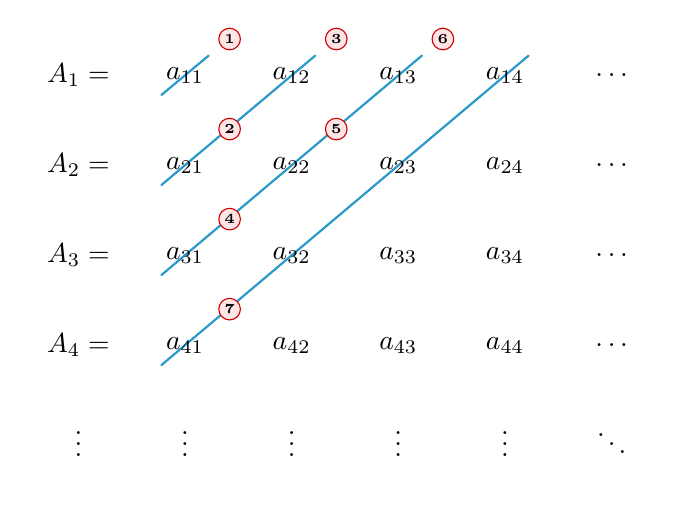
\begin{tikzpicture}[
    chalkLine/.style={thick, cyan!80!black, line cap=round}, % 斜线样式（模拟黑板上的粉笔斜划线）
    numBadge/.style={circle, fill=red!10, draw=red!80!black, inner sep=1pt, font=\tiny\bfseries}, % 右上角编号小标记
]
    % 1. 构建二维矩阵网格
    \matrix (m) [
        matrix of math nodes,
        nodes={anchor=center, minimum width=3em, minimum height=2.4em, inner sep=2pt},
        column sep=0.3cm,
        row sep=0.3cm
    ] {
        A_1 = & a_{11} & a_{12} & a_{13} & a_{14} & \dots \\
        A_2 = & a_{21} & a_{22} & a_{23} & a_{24} & \dots \\
        A_3 = & a_{31} & a_{32} & a_{33} & a_{34} & \dots \\
        A_4 = & a_{41} & a_{42} & a_{43} & a_{44} & \dots \\
        \vdots & \vdots & \vdots & \vdots & \vdots & \ddots \\
    };

    % 2. 在背景层绘制贯穿元素的斜线（板书同款划法）
    \begin{scope}[on background layer]
        \draw[chalkLine] ([shift={(-0.3,-0.25)}]m-1-2.center) -- ([shift={(0.3,0.25)}]m-1-2.center);
        \draw[chalkLine] ([shift={(-0.3,-0.25)}]m-2-2.center) -- ([shift={(0.3,0.25)}]m-1-3.center);
        \draw[chalkLine] ([shift={(-0.3,-0.25)}]m-3-2.center) -- ([shift={(0.3,0.25)}]m-1-4.center);
        \draw[chalkLine] ([shift={(-0.3,-0.25)}]m-4-2.center) -- ([shift={(0.3,0.25)}]m-1-5.center);
    \end{scope}

    % 3. 标注自然数编号顺序 (1, 2, 3, 4, 5, 6...)
    \node[numBadge, above right=-2pt and -2pt of m-1-2] {1};
    \node[numBadge, above right=-2pt and -2pt of m-2-2] {2};
    \node[numBadge, above right=-2pt and -2pt of m-1-3] {3};
    \node[numBadge, above right=-2pt and -2pt of m-3-2] {4};
    \node[numBadge, above right=-2pt and -2pt of m-2-3] {5};
    \node[numBadge, above right=-2pt and -2pt of m-1-4] {6};
    \node[numBadge, above right=-2pt and -2pt of m-4-2] {7};
\end{tikzpicture}
\end{document}